\documentclass[11pt, a4paper]{scrartcl}
\usepackage[ngerman]{babel}
%\usepackage[T1]{fontenc}
\usepackage[utf8]{inputenc}
\usepackage{lmodern}
\usepackage{amsmath}
\usepackage{amssymb}
\usepackage{amsthm}
\usepackage{graphicx}
\usepackage{listings}
\usepackage{booktabs}
\usepackage{float}
\usepackage{pdfpages}
\usepackage{cite}
\usepackage{url}
\bibliographystyle{unsrtnat}
\usepackage[numbers]{natbib}
\usepackage[T1]{fontenc}
%
\begin{document}
\lstset{basicstyle=\small,
		 inputencoding=latin1,
		stringstyle=\ttfamily,
		identifierstyle=,
		showstringspaces=false,
		language=c,
		frame=trBL,
		numbers=left,
		numberstyle=\footnotesize
		}
%
\subsection*{TI III WS 2013, Fr. 12-14}
\section*{Lösung Übungsblatt 8}
\textbf{Christoph van Heteren-Frese (Matr.-Nr.: 4465677), Julien  Stengel } \\%(Matr.-Nr.: 4567553)}\\
Tutor: Ruhland, eingereicht am \today\\
\hrule
%
\section*{Aufgabe 3}
Als Bufferoverlow wird eine Sicherheitslücke bezeichnet, bei der zu große Datenmengen in einen dafür zu kleinen reservierten Speicherbereich geschrieben werden. Als Konsequenz werden die hinter dem Ziel-Speicherbereich liegenden Speicherstellen überschrieben.
Gelingt es auf diese Weise Rücksprungadressen von Funktionen zu überschreiben, kann somit fremder Code eingeschleust und ausgeführt werden.
\subsubsection*{Beispiel:}
\lstinputlisting[captionpos=b,caption=overflow.c, label=overflow]{../overflow.c}
Das Beispiel in Listing \ref{overflow} verdeutlicht die Gefahr, die von einem Bufferoverflow ausgehen kann. Es wird eine Eingabe unbestimmter Länge gelesen. Ist die Eingabe länger als ein Zeichen, wird die Variable \texttt{access} überschrieben	. Dies führt zur Verfälschung einer Sicherheitsüberprüfung.
\section*{Aufgabe 4}
\subsection*{a)}
\begin{quote}
\texttt{PRINT\_INTEGER(square(1+1));}
\end{quote}
in Zeile 17 von Listing \ref{label} wird durch den Präprozessor durch 
\begin{quote}
\texttt{printf("\%d ",1+1*1+1);;}
\end{quote}
ersetzt. Da \texttt{*} stärker bindet als \texttt{+} wird der Ausdruck \texttt{1+1*1+1} zu \texttt{3} ausgewertet. 

\subsection*{b)}
\begin{quote}
\texttt{\#define isdigit(c) (c>='0' \&\& c<='9') ? 1 : 0}
\end{quote}
Siehe auch Listing \ref{label} Zeile 7.
\subsection*{c)}
\begin{quote}
\texttt{printf("\textbackslash nMaximum von a und b: \%d\textbackslash n",max(a,b++));}
\end{quote}
in Zeile 22 von Listing \ref{label} wird durch den Präprozessor durch 
\begin{quote}
\texttt{printf(" \textbackslash nMaximum von a und b: \%d \textbackslash n",(a>b++) ? a : b++);}
\end{quote}
ersetzt. Der Ausdruck \texttt{(a>b++) ? a : b++} inkrementiert den Wert von \texttt{b} zwei Mal: einmal direkt nach dem Vergleich (dieser Wert wird direkt ausgegeben) und das zweite Mal nach der Ausgabe. Somit ist der Wert bei der zweiten Ausgabe zwei Mal erhöht.
\subsection*{d)} 
\textbf{Vorteile} von Makros liegen in der besseren Performance, die sich in einer Leistungssteigerung und einer kürzeren Laufzeit bemerkbar macht: Wird z.B. die Hälfte des Quelltextes bereits durch den Prozessor bearbeitet, ist nur noch die andere Hälfte vom Compiler zu bearbeiten. Ein weiterer Vorteil ist die ermöglichte Verbesserung der Lesbarkeit.\\\\
\textbf{Nachteile}: Der Leisterungssteigerung von Makros steht der erhöhte Speicherverbrauch entgegen.  Des weiteren erhöht sich die Anzahl der möglichen Fehlerquellen. 
\subsection*{e)}
Es wird \texttt{VERBOSE nicht definiert} ausgegeben (an Stelle von \texttt{Test zu Ende!}, wenn die Zeile \texttt{\#define VERBOSE} nicht entfernt wird).\\
\textbf{Begründung:} Mit der Präprozessoranweisung
\begin{quotation}
\noindent \texttt{\#ifdef VERBOSE}
%  printf("Test zu Ende!\textbackslash n");\\
%\#else\\
%  printf("VERBOSE nicht definiert\textbackslash n");\\
%\#endif}
\end{quotation}
in Zeile 26 wird abgefragt, ob das Symbol \texttt{VERBOSE} definiert wurde oder nicht. Ist das der Fall, wird der Block im Anschluß ausgeführt. Wenn das Symbol
nicht definiert ist, wird der Block nach \texttt{\#else} (Zeile 28) ausgeführt, so dass die oben genannte Ausgabe entsteht.
\vspace{1cm}
\lstinputlisting[captionpos=b,caption=u8\_4.c, label=label]{../u8_4.c}
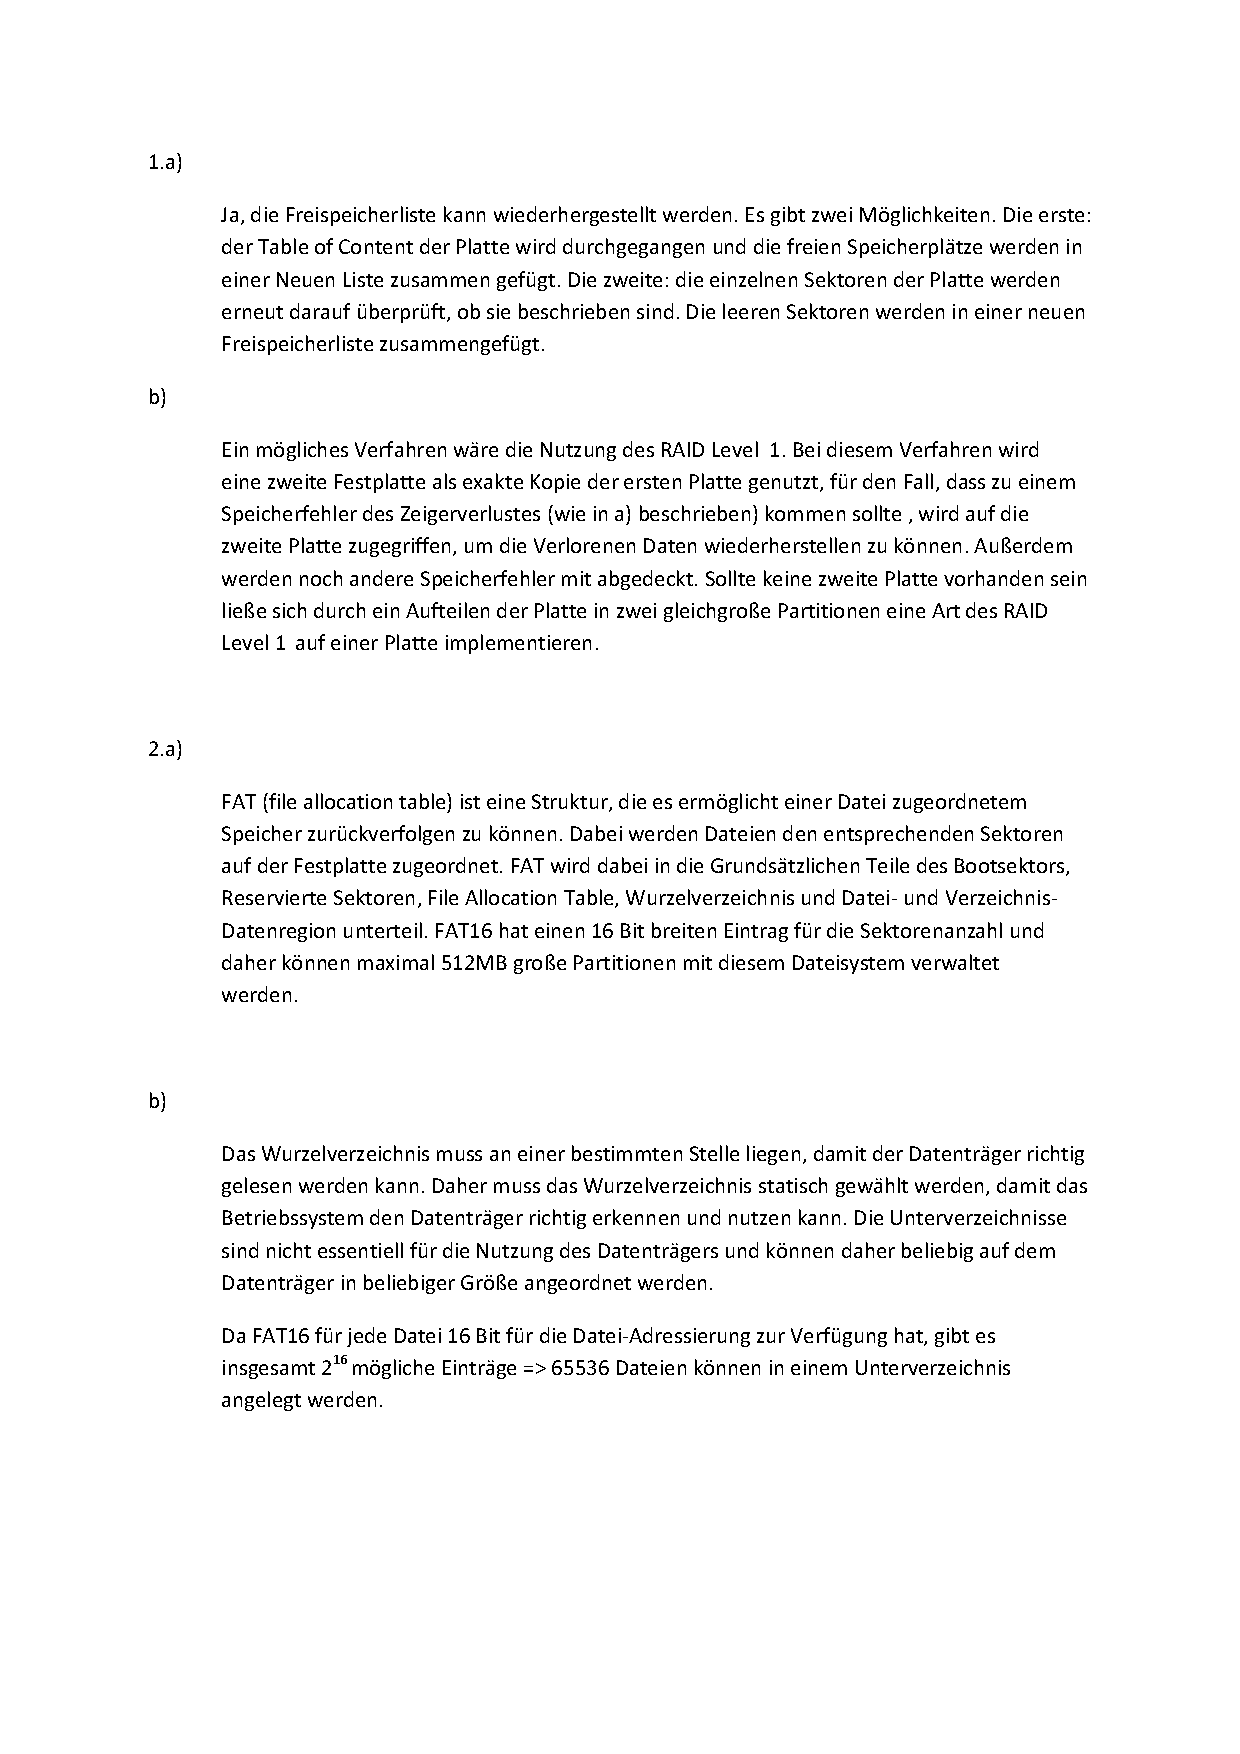
\includepdf[pages={1}]{../uebung_8.pdf}
\bibliography{ti3}
\end{document}
